\documentclass[a4paper]{article}

\usepackage{graphicx}
\usepackage{amsmath,amssymb}
\usepackage{minted}
\usepackage{multirow}
\usepackage{float}
\usepackage{algorithm}
\usepackage{algpseudocode}
\usepackage{todonotes}
\usepackage{forest}
\usepackage{xstring}
\usepackage{xcolor}
\usepackage[most]{tcolorbox}
\usepackage{xparse}
\usepackage{natbib}
\usepackage{adjustbox}

\usetikzlibrary{graphs,graphdrawing}
\usegdlibrary{layered}

% for external graphviz
\input{/home/donkarlo/Dropbox/repo/nd_language_ai_project/src/nd_language_ai/formal/computer/programming/tex/latex/code_clips/external_graphviz.tex}

% for tags
\input{/home/donkarlo/Dropbox/repo/nd_language_ai_project/src/nd_language_ai/formal/computer/programming/tex/latex/part/control_sequence/kind/semtag/semtag.tex}

% for links
\input{/home/donkarlo/Dropbox/repo/nd_language_ai_project/src/nd_language_ai/formal/computer/programming/tex/latex/code_clips/seehere.tex}

% for nested lists and sections
\input{/home/donkarlo/Dropbox/repo/nd_language_ai_project/src/nd_language_ai/formal/computer/programming/tex/latex/code_clips/deep_structure.tex}

\title{Prediction and state estimation}
\date{}
\author{Mohammad Rahmani}

\begin{document}
   \maketitle

   \section{Motion model}
      \seeherefooter{/nd_robotic_ai_learning_project/src/robot/part/mind/cognition/part/object_level/process/part/perception/state_estimation/model/motion_model/motion_model.tex}
      A motion model describes how the state of a robot changes over time as a result of motion or control input. In probabilistic robotics, it is commonly used to predict the next robot state during localization and state estimation \cite{thrun-2005-probabilistic-robotics}.

      A general probabilistic motion model can be written as
      \[
      p(x_k \mid x_{k-1},u_k),
      \]
      where $x_{k-1}$ is the previous state, $u_k$ is the motion or control input, and $x_k$ is the predicted current state.


      This research uses the quasi-constant velocities derived from the vowels as described in Section \ref{neural_cognitive_architecture}

   \section{Grandmother neurons}
      A grandmother cell is a hypothetical neuron that represents a complex but specific concept, object, or individual \cite{gross-2002-genealogy-of-the-grandmother-cell, quiroga-2005-invariant-visual-representation-by-single-neurons-in-the-human-brain}.

      In this research all mathematical approaches for which no neural representation exists, a grand mother cell is used
      \subsection{Bayesian brain}
         To see bayesian brain theories \seeherefooter{/nd_robotic_ai_learning_project/src/robot/part/body/part/nervous_system/part/central/brain/theory/kind/bayesian/bayesian.tex}

         \subsubsection{Velocity motion model}


            A velocity motion model predicts the next state from commanded or measured translational and rotational velocities \cite{thrun-2005-probabilistic-robotics}.

            For a planar robot with pose
            \[
            x_k =
            \begin{bmatrix}
               x_k & y_k & \theta_k
            \end{bmatrix}^{T},
            \]
            and control input
            \[
            u_k =
            \begin{bmatrix}
               v_k & \omega_k
            \end{bmatrix}^{T},
            \]
            a simple discrete kinematic approximation is
            \[
            x_k =
            x_{k-1}
            +
            \begin{bmatrix}
               v_k\cos\theta_{k-1}\\
               v_k\sin\theta_{k-1}\\
               \omega_k
            \end{bmatrix}
            \Delta t.
            \]

            This model is useful when linear and angular velocity commands or measurements are directly available.
         \subsubsection{Kalman filter}
            \cite{kalman-1960-a-new-approach-to-linear-filtering-and-prediction-problems}
            is used in this research as in the literature it  is shown to be practiced in brain               \cite{wolpert-2007-probabilistic-models-in-human-sensorimotor-control}. It fuses latest Gaussian observation (derived from intensity rat esensor) with Gaussian prediction . This research uses it for fusing Gaussian transformer  in section \ref{guassian_tranfsomrer} together with agent's velocity derived from second derivative (intensity change rate sensor) to make predictions along time.

         \subsubsection{Particle filter}
            \seeherefooter{/nd_robotic_ai_learning_project/src/robot/part/mind/cognition/part/object_level/process/part/perception/state_estimation/slam/kind/particle_filter/particle_filter.tex}
            \cite{arulampalam-2002-a-tutorial-on-particle-filters-for-online-nonlinear-non-gaussian-bayesian-tracking} describes the particle filter as a sequential Monte Carlo method that represents a probability distribution by a finite set of weighted samples called particles. In this research it is used to assign a Gaussian distribution at each level at any abstract level.

            Particle filter is shown by researchers such as
            \cite{kutschireiter-2017-nonlinear-bayesian-filtering-and-learning-a-neuronal-dynamics-for-perception} to be used in human brain for state estimation.


         \subsubsection{Gaussian transformer(GTF)} \label{guassian_tranfsomrer}
            \seeherefooter{
            /nd_datascience_learning_project/src/machine_learning/model/architecture/neural_network/kind/deep_learning/kind/transformer/kind/uncertainty/uncertainty.tex}
            A multi attention head gaussian transformer is used in this research to make predictions.

            A multi attention predictor is needed. The transformers \cite{vaswani-2017-attention-is-all-you-need}

            Its application here is to replace the constant speed predictor



            \begin{itemize}
               \item At lowest level in each cell, it holds an AP wave represented by FMM
               \item Training
               \begin{itemize}
                  \item Deep learning as an autocorrelation to find periods
               \end{itemize}
               \item Sliding windows to train the transformer
               \item Period sampling with auto correlation for training and validating the transformer
               \item Noise as uncertainty in transformer

            \end{itemize}
            \paragraph{Gaussian Transformer}
               The model receives a past time-series window and predicts a future window with uncertainty.



               \[
               f_{\theta}:
               \mathbb{R}^{T_{\mathrm{in}} \times F_{\mathrm{in}}}
               \rightarrow
               \mathbb{R}^{T_{\mathrm{out}} \times 2F_{\mathrm{out}}}
               \]



               For each future time step and feature, it predicts two values:

               \[
               \hat{Y}_{\mathrm{params}}
               =
               [
               \mu,
               \log \sigma^2
               ]
               \]



               \[
               y_{b,t,j}
               \sim
               \mathcal{N}
               (
               \mu_{b,t,j},
               \sigma^2_{b,t,j}
               )
               \]



               \begin{itemize}
                  \item \(\mu\): expected future value
                  \item \(\sigma^2 = \exp(\log \sigma^2)\): predictive uncertainty
               \end{itemize}
            \paragraph{Loss function for gaussian transformer to interpret uncertainty}
               The model is trained with Gaussian negative log-likelihood:

               \[
               \mathcal{L}
               =
               \frac{1}{BT_{\mathrm{out}}}
               \sum_{b=1}^{B}
               \sum_{t=1}^{T_{\mathrm{out}}}
               \sum_{j=1}^{F_{\mathrm{out}}}
               \frac{1}{2}
               \left[
               \log \sigma^2_{b,t,j}
               +
               (y_{b,t,j}-\mu_{b,t,j})^2
               \exp
               (
               -\log \sigma^2_{b,t,j}
               )
               \right]
               \]



               Approximate 95 percent prediction interval:

               \[
               y_{b,t,j}
               \in
               [
               \mu_{b,t,j}
               -
               1.96\sigma_{b,t,j},
               \mu_{b,t,j}
               +
               1.96\sigma_{b,t,j}
               ]
               \]



               Small variance means high confidence. Large variance means high uncertainty.

   \section{Joint PF--GTF prediction and KF state estimation}
      \begin{figure}[H]
         \centering
         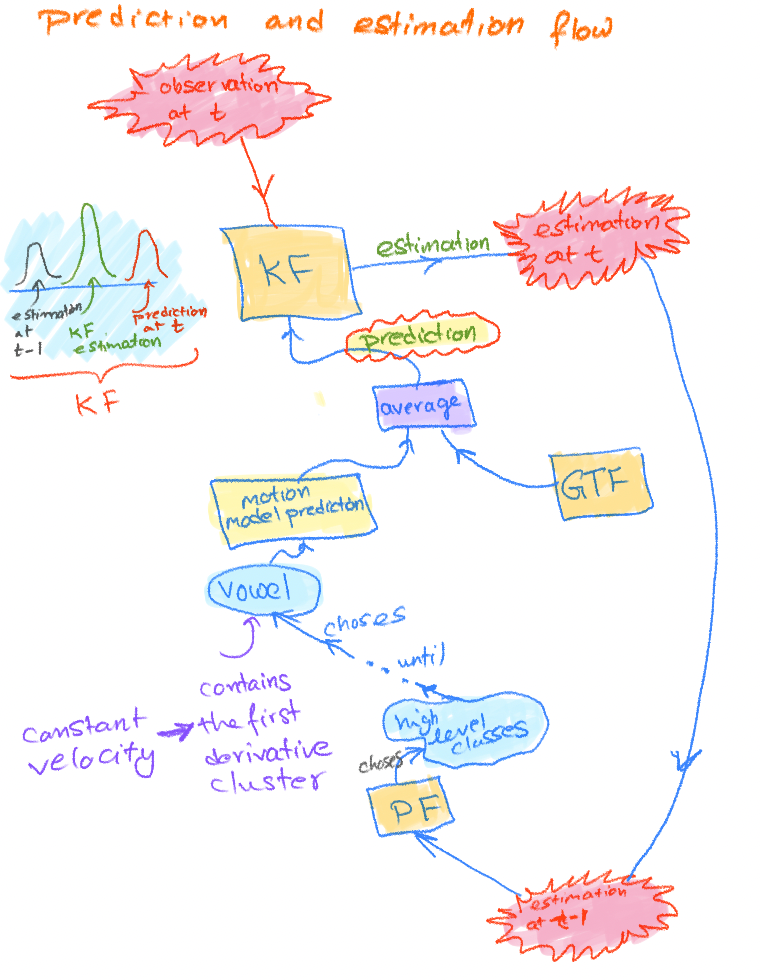
\includegraphics[width=0.9\textwidth]{prediction_and_state_estimation_model.png}
      \end{figure}

      Let \(\hat{\mathbf{x}}_{t-1}\) denote the state estimate at time \(t-1\). In this architecture, this estimate is the recurrent state input to the particle filter (PF). The state is represented by AP-FMM parameters, and the PF propagates weighted hypotheses through the successive representation levels. At each level \(\ell\), the particles induce probabilities over the learned classes,
      \[
      \pi_{t,k}^{(\ell)}
      =
      p\!\left(C_k^{(\ell)}\mid \hat{\mathbf{x}}_{t-1},\mathcal{Y}_{1:t-1}\right),
      \qquad
      \sum_k \pi_{t,k}^{(\ell)}=1.
      \]
      The propagation continues through the hierarchy until the vowel level is reached. In this research, a vowel represents the first derivative of the AP-FMM parameters and therefore provides the velocity-like quantity used by the motion model.

      For a vowel class \(C_k^{(v)}\) containing \(N_k\) learned velocity observations \(\mathbf{v}_{k,j}\), the class is retained as its empirical distribution rather than being reduced to a single centroid,
      \[
      \mu_k^{(v)}
      =
      \frac{1}{N_k}\sum_{j=1}^{N_k}\delta_{\mathbf{v}_{k,j}}.
      \]
      Consequently, the PF prediction at the vowel level is the class-probability-weighted empirical mixture
      \[
      p_{\mathrm{PF}}(\mathbf{v}_t)
      =
      \sum_k \pi_{t,k}^{(v)}\mu_k^{(v)}(\mathbf{v}_t).
      \]
      Each velocity hypothesis propagates the previous estimate through the motion model \(g(\cdot)\),
      \[
      \mathbf{x}_{t}^{(k,j)}
      =
      g\!\left(\hat{\mathbf{x}}_{t-1},\mathbf{v}_{k,j},\Delta t\right),
      \]
      yielding the PF predictive state distribution
      \[
      p_{\mathrm{PF}}(\mathbf{x}_t\mid\hat{\mathbf{x}}_{t-1})
      =
      \sum_k\frac{\pi_{t,k}^{(v)}}{N_k}
      \sum_{j=1}^{N_k}
      \delta_{\mathbf{x}_{t}^{(k,j)}}.
      \]

      In parallel, the Gaussian Transformer (GTF) uses the preceding AP-FMM time-series window and produces a probabilistic forecast
      \[
      p_{\mathrm{GTF}}(\mathbf{x}_t)
      =
      \mathcal{N}\!\left(
      \boldsymbol{\mu}_{t}^{\mathrm{GTF}},
      \mathbf{P}_{t}^{\mathrm{GTF}}
      \right).
      \]
      Thus, the PF contributes the hierarchical class-conditioned motion prediction, whereas the GTF contributes the learned temporal prediction and its uncertainty.

      The two predictions are combined by an equal-weight linear opinion pool (mixture average),
      \[
      p_t^{-}(\mathbf{x})
      =
      \frac{1}{2}p_{\mathrm{PF}}(\mathbf{x})
      +
      \frac{1}{2}p_{\mathrm{GTF}}(\mathbf{x}).
      \]
      Because the Kalman update requires a Gaussian prior, this mixture is moment-matched to a Gaussian. Let \((\boldsymbol{\mu}_{t}^{\mathrm{PF}},\mathbf{P}_{t}^{\mathrm{PF}})\) be the weighted mean and covariance of the PF predictive particles. Then
      \[
      \hat{\mathbf{x}}_{t}^{-}
      =
      \frac{1}{2}\boldsymbol{\mu}_{t}^{\mathrm{PF}}
      +
      \frac{1}{2}\boldsymbol{\mu}_{t}^{\mathrm{GTF}},
      \]
      and
      \[
      \mathbf{P}_{t}^{-}
      =
      \frac{1}{2}\!\left[
      \mathbf{P}_{t}^{\mathrm{PF}}
      +(\boldsymbol{\mu}_{t}^{\mathrm{PF}}-\hat{\mathbf{x}}_{t}^{-})
      (\boldsymbol{\mu}_{t}^{\mathrm{PF}}-\hat{\mathbf{x}}_{t}^{-})^{T}
      \right]
      +
      \frac{1}{2}\!\left[
      \mathbf{P}_{t}^{\mathrm{GTF}}
      +(\boldsymbol{\mu}_{t}^{\mathrm{GTF}}-\hat{\mathbf{x}}_{t}^{-})
      (\boldsymbol{\mu}_{t}^{\mathrm{GTF}}-\hat{\mathbf{x}}_{t}^{-})^{T}
      \right].
      \]
      The resulting \(\mathcal{N}(\hat{\mathbf{x}}_{t}^{-},\mathbf{P}_{t}^{-})\) is the prediction supplied to the Kalman filter.

      The observation at time \(t\), denoted by \(\mathbf{y}_t\), is also represented in AP-FMM parameter space. With observation model
      \[
      \mathbf{y}_t
      =
      \mathbf{H}_t\mathbf{x}_t+\boldsymbol{\nu}_t,
      \qquad
      \boldsymbol{\nu}_t\sim\mathcal{N}(\mathbf{0},\mathbf{R}_t),
      \]
      the Kalman correction is
      \[
      \mathbf{S}_t
      =
      \mathbf{H}_t\mathbf{P}_t^{-}\mathbf{H}_t^{T}+\mathbf{R}_t,
      \qquad
      \mathbf{K}_t
      =
      \mathbf{P}_t^{-}\mathbf{H}_t^{T}\mathbf{S}_t^{-1},
      \]
      \[
      \boxed{
      \hat{\mathbf{x}}_t
      =
      \hat{\mathbf{x}}_t^{-}
      +
      \mathbf{K}_t
      \left(
      \mathbf{y}_t-\mathbf{H}_t\hat{\mathbf{x}}_t^{-}
      \right)}
      \]
      and
      \[
      \mathbf{P}_t
      =
      (\mathbf{I}-\mathbf{K}_t\mathbf{H}_t)\mathbf{P}_t^{-}.
      \]
      Therefore, \(\hat{\mathbf{x}}_t\) is the final state estimate at time \(t\). It is fed back as \(\hat{\mathbf{x}}_{t-1}\) in the next time step, closing the recursive PF--GTF--KF prediction and state-estimation loop.

      \bibliographystyle{plainnat}
      \bibliography{/home/donkarlo/Dropbox/repo/nd_shared_research/bibliography/bibliography.bib}
\end{document}
